%%=============================================================================
%% Inleiding
%%=============================================================================

\chapter{\IfLanguageName{dutch}{Inleiding}{Introduction}}%
\label{ch:inleiding}


\section{\IfLanguageName{dutch}{Probleemstelling}{Problem Statement}}%
\label{sec:probleemstelling}

In de zorgindustrie wordt er steeds meer gesproken over 'alarmmoeheid'. Volgens \textcite{Ferrara2023} kan alarmmoeheid worden omschreven als ''een overprikkeling of zintuiglijke overbelasting, in staat tot het veroorzaken van gevoelloosheid ten opzichte van alarmen door een te groot aantal alarmen die foutief of klinisch onbelangrijk zijn.'' De ernst van de gevolgen van deze moeheid is verontrustend. Zo stelt \textcite{Ferrara2023} dat de gedragsmatige reactie van het verplegend personeel, dat lijdt aan een hoge alarmmoeheid, ongepast is. Deze reacties variëren tussen het geluid van het alarmsignaal aanpassen en volledige uitschakeling van het alarm., wat dus een mogelijk gevaar voor de patiënt inhoudt. Deze stelling wordt bevestigd door het onderzoek van \textcite{Casey2018}. Uit hun onderzoek kwam naar voren dat 90,2 \% van het geïnterviewde verplegend personeel, oordeelt dat foutieve of klinisch onbelangrijke alarmen frequent voorkomen, de patiëntenzorg verstoren en het vertrouwen in het alarmsysteem beschadigen. Verder zou tot 80,5\% van het geïnterviewde verplegend personeel, het alarmsysteem soms deactiveren.
\\\\
Twee van de onderdelen van dit alarm-/monitoringsysteem zijn het \gls{dect}-systeem en het personenalarm. Het \gls{dect}-systeem is het audiosysteem dat gebruikmaakt van een mobiel toestel om binnen een bedrijf, in deze situatie een ziekenhuis, tussen diensten en personeel te communiceren. Hoewel het systeem al een hele tijd bestaat, sinds 1993, zijn er toch enkele gebreken. Zo is er interferentie met andere medische apparatuur, dekkingsbeperkingen en de gelimiteerde functionaliteit. Deze functionaliteit is net gelimiteerd door het type communicatiesysteem het is, zo is er enkel audiosysteem is. De laatste zou een update/upgrade kunnen gebruiken om visuele ondersteuning te bieden aan het personeel.
In tegenstelling tot het \gls{dect}-systeem, ligt het personenalarm volledig bij de patiënt. Deze is in bezit van een alarmknop waarmee hulp kan worden opgeroepen. Deze alarmsignalen kunnen ook foutief zijn, en zo bijdragen aan de alarmmoeheid.\\

Volgens \textcite{Coiera2006} bestaat de informatie-uitwisseling in gezondheidszorg voornamelijk uit communicatie tussen personen. Dit wordt een ''Communication space'' genoemd. Dit omvat onder andere conversaties via telefoon en in persoon, e-mails, brieven, \ldots . Verder wijst het onderzoek van \textcite{Coiera2006} aan dat de complexiteit van conversaties stijgt naarmate er meer mensen betrokken raken. Dit komt omdat er verschillende conversaties tussen 2 personen kunnen gevoerd worden.

\begin{figure}[H]
  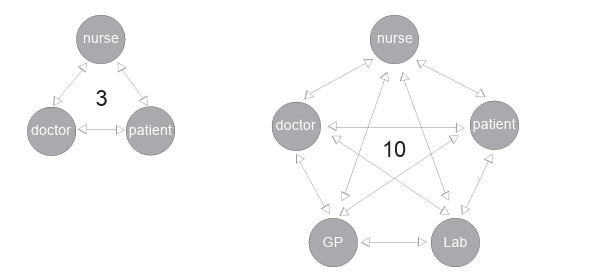
\includegraphics[width=\linewidth]{../graphics/Number-of-conversations.png}
  \caption{Aantal mogelijke conversaties stijgt samen met het aantal personen dat deelneemt aan communicatie. \autocite[Uit ''Communication Systems in Healthcare'' door][The Clinical Biochemist Reviews, 27(2) , 90.]{Coiera2006} Copyright 2006 van \textcite{Coiera2006}}
  \label{fig:aantal conversaties}
\end{figure}

\section{\IfLanguageName{dutch}{Onderzoeksvraag}{Research question}}%
\label{sec:onderzoeksvraag}

Het is de combinatie van de stijging in complexiteit van informatie uitwisselen met de nadelen van het \gls{dect}-systeem en de gevaren van alarmmoeheid die ervoor zorgt dat het huidige systeem wordt in vraag getrokken. Zo bekomen we ook de hoofdvraag die wordt behandeld in deze bachelorproef: \textit{''Hoe kan de informatie-uitwisseling tussen artsen en verplegend personeel in ziekenhuizen verbeterd worden door het inzetten van nieuwe technologieën''}.\\
Deze bachelorproef zal focussen op het onderzoeken van welke innovaties een waardevol alternatief kunnen zijn voor het \gls{dect}-systeem. Dit onderzoek is gericht op IT-personeel in gezondheidszorginstituten.\\\\

\begin{enumerate}
  \item \textit{Wat zijn de kenmerken van het \gls{dect}-systeem?}
  \item \textit{Wat is het huidige systeem (met \hyphenation{rand-apparatuur}randapparatuur) en wat zijn de nadelen hiervan?}
  \item \textit{Hoe kan een zorgsituatie worden gesimuleerd?}
  \item \textit{Welke pogingen zijn al ondernomen om het \gls{dect}-systeem als standaard aan te passen?}
  \item \textit{Wat zijn de minimumvereisten voor technologieën, om als alternatief te kunnen worden beschouwd?}
  \item \textit{Welke andere communicatiemogelijkheden zijn er die voldoen aan de minimumvereisten?}
  \item \textit{Welke mogelijke data-integratie mogelijkheden hebben de alternatieven?}
  \item \textit{Welke eigenschappen van het alternatief hebben een vermindering in alarmmoeheid als gevolg?}
  \item \textit{Vanaf wanneer is het haalbaar om te implementeren op economisch vlak?}
\end{enumerate}

\section{\IfLanguageName{dutch}{Onderzoeksdoelstelling}{Research objective}}%
\label{sec:onderzoeksdoelstelling}

%TODO:

Het beoogde resultaat van deze bachelorproef is een \gls{poc}. Deze is een simulatie met verduidelijking van de verdere stappen om een omzetting van de simulatie naar praktijk te realiseren. De criteria voor succes zijn de minimum vereisten, zie hoofdstuk~\ref{sec:req}.

\section{\IfLanguageName{dutch}{Opzet van deze bachelorproef}{Structure of this bachelor thesis}}%
\label{sec:opzet-bachelorproef}

De proof of concept die wordt opgesteld tijdens de bachelorproef is in samenwerking met Citymesh\footnote{https://www.citymesh.com/} en met 360° Zorglab\footnote{https://www.hogent.be/projecten/zorglab/}. Citymesh is een bedrijf dat zich specialiseert in connectiviteit, met focus op permanente en tijdelijke netwerkinfrastructuur. Dit door gebruik te maken van Wi-Fi, 0G-, 4G- en 5G-technologieën \autocite{Citymesh2024}. Het 360° Zorglab is een project van HOGENT. De kern van het Zorglab is het creëren van een wisselwerking tussen disciplines enerzijds en tussen onderzoek, dienstverlening en onderwijs anderzijds. Toekomstige gezondheids- en welzijnsmedewerkers kunnen hier in een veilige omgeving niet-technische skills aanleren in een interprofessionele context. \autocite{HOGENT2024} Het doel van deze samenwerking is een snelle wisselwerking te kunnen creëren om zo meerdere malen de testfases te kunnen doorlopen. 

% Het is gebruikelijk aan het einde van de inleiding een overzicht te
% geven van de opbouw van de rest van de tekst. Deze sectie bevat al een aanzet
% die je kan aanvullen/aanpassen in functie van je eigen tekst.

De rest van deze bachelorproef is als volgt opgebouwd:

In Hoofdstuk~\ref{ch:stand-van-zaken} wordt een overzicht gegeven van de stand van zaken binnen het onderzoeksdomein, op basis van een literatuurstudie.\\
In Hoofdstuk~\ref{ch:methodologie} wordt de methodologie toegelicht en worden de gebruikte onderzoekstechnieken besproken om een antwoord te kunnen formuleren op de onderzoeksvragen.\\
In Hoofdstuk~\ref{ch:poc} wordt de eerste \gls{poc} uitgelegd en aangetoond hoe deze tot stand is gekomen met de code. Deze wordt ook in dit hoofdstuk geëvalueerd en een tussentijds resultaat zal worden opgesteld.\\
In Hoofdstuk~\ref{ch:conclusie} wordt de conclusie gegeven en een antwoord geformuleerd op de onderzoeksvragen. Daarbij wordt ook een aanzet gegeven voor toekomstig onderzoek binnen dit domein.\\
Als laatste worden de bijlagen toegevoegd. Deze bevatten het originele voorstel van de bachelorproef (Bijlage \ref{ch:voorstel}), installatiegids (Bijlage \ref{ch:InstallationGuide}), en automatisatie scripts (Bijlage \ref{ch:vagrant}).